\documentclass[journal]{IEEEtran}

\usepackage{bm,cite,algorithm,algorithmic,float,amsmath,amssymb}

\usepackage{amssymb}
\usepackage{amsmath}
\usepackage{graphicx}
\usepackage{cite}
%\usepackage{citesort}
%\usepackage[utf8x]{inputenc}
\usepackage{amsthm}
\usepackage{framed}
\usepackage{url}
%\newtheorem{definition}{Definition}
\newtheorem{theorem}{Theorem}
\newtheorem{lemma}{Lemma}
\newtheorem{proposition}{Proposition}
\newtheorem{axiom}{Axiom}
\newtheorem{corollary}{Corollary}
\newtheorem{remark}{Remark}
\newtheorem{example}{Example}
\newtheorem{property}{Property}
\newtheorem{definition}{Definition}
\newtheorem{hypothesis}{Hypothesis}
%\bibliographystyle{IEEEtran}
\IEEEoverridecommandlockouts

\newcommand{\defequal}{\mbox{$\stackrel{\triangle}{=}$}}

\usepackage{graphicx,epstopdf}
\usepackage{epsfig}	
\usepackage{amsfonts}
%\usepackage{bbm}
\floatname{algorithm}{Algorithm}
\newcommand{\EX}[1]{\mathbb{E}\left\{{#1}\right\}}
\newcommand{\EXs}[2]{\mathbb{E}_{{#1}}\left\{{#2}\right\}}
\newcommand{\PDF}[2]{f_{{#1}}\left({#2}\right)}
\newcommand{\CDF}[2]{F_{{#1}}\left({#2}\right)}
\newcommand{\CCDF}[2]{C_{{#1}}\left({#2}\right)}
% for binomial coefficients (AmS-LaTeX)
%\newcommand{\bc}[2]{\genfrac{(}{)}{0pt}{}{#1}{#2}}
\newcommand{\bc}[2]{{}_{#1}C_{#2}}
\newcommand{\BG}[2]{\bar{{#1}}_{{#2}}}
\newcommand{\TG}[1]{\tilde{{#1}}}

\newcommand{\A}[1]{(\textbf{A#1:})}

%\newcounter{mytempeqncnt}

\DeclareMathOperator*{\argmax}{argmax}
\DeclareMathOperator*{\argmin}{argmin}

\hyphenation{op-tical net-works semi-conduc-tor}
\raggedbottom
\begin{document}
	
	\title{Goal-Oriented $1$-Bit Quantization With Uncertain Distortion Measures\thanks{M. Egan is with Univ Lyon, INRIA, INSA Lyon, CITI, France (email: malcom.egan@inria.fr). This work was partially supported by the French National Agency for Research (ANR) via the project ANR-22-PEFT-0010 of the France 2030 program PEPR réseaux du Futur, and the project ANR-24-CE25-2256 TCDTP.}}
	
	% for a Family of Non-Separable Distortion Criteria}

\author{Malcolm Egan}
%{$^1$\footnotesize INSA}\\
%{$^2$\footnotesize INRIA}\\
%{$^3$\footnotesize Faculty of Electrical Engineering, Czech Technical University in Prague}}

\maketitle

\begin{abstract}
Tailoring low resolution quantization to specific tasks is an important aspect of goal-oriented communications, with applications ranging from channel state information feedback for MIMO systems to compression of neural network weights. However, target distortion functions associated with a task may either be imperfectly known or intractable to compute. In these cases, there is uncertainty in the distortion function. In this paper, we propose new criteria based on risk measures to design $1$-bit quantizers with uncertainty in the distortion function. While information-theoretic limits of compression with risk measure constraints have recently been established, quantizers based on risk measure criteria have not yet been developed. We introduce an algorithm for quantizer design with our risk measure criteria based on the cross-entropy method, and apply our approach to an environmental monitoring dataset. 
\end{abstract}


\maketitle

\section{Introduction}

Low resolution quantization plays an important role in communications and learning. For example, channel feedback for MIMO at mmWave frequencies requires quantizers with only a small number of a bits, or even a single bit \cite{Mo2015capacity}. In compression of large deep neural networks for memory-constrained devices, neuron weights are also compressed with a low resolution quantizer \cite{Nahshan2021loss}. 

The choice of a quantizer depends on the probability distribution of the data, and a measure of distortion between the data samples and their quantizations. For real-valued data, a standard choice of the distortion measure is the mean-square error \cite{Gersho2012vector}. However, the choice of the mean-square error is largely due to its simplicity and the fact that many distortion measures are Lipschitz continuous and therefore can be bounded in terms of the Euclidean norm. Indeed, application-dependent measures of distortion can yield improved performance in what is often known as goal- or task-oriented compression \cite{Gunduz2022beyond}. For example, in speech compression the mean distortion measures based on the $p$-norm, weighted square error amongst others are common alternatives to the mean-square error \cite{Linde1980algorithm}. In \cite{Zou2022goal}, the mean optimality loss has been considered for resource allocation problems, and in \cite{Nahshan2021loss} mean $p$-norm distortion functions have been applied for compression of neural network weights. 

% When application-dependent norms don't work properly
Goal-oriented quantization can outperform quantizer based on the mean-square error, but only when the distortion measure is appropriately tailored to a target application. In speech and vision applications, a target distortion measure often is based on human visual or aural perception experiments \cite{Jayant1993signal,Eckert1998perceptual}. Measurements in these experiments are often imperfect, resulting in uncertainty in the quality of the distortion measure. In the context of resource allocation problems, the mean optimality loss may an appropriate distortion measure \cite{Zou2022goal}. However, it can be extremely costly to evaluate the optimality loss for a large number of samples. As such, approximations of the optimality loss may be required to construct quantizers by, for example, Lloyd-type algorithms \cite{Linde1980algorithm}. As for speech and vision applications, there is uncertainty in the quality of the distortion measure.

% How to account for uncertainty in the distortion function
In this paper, we propose a method to select a quantizer when there is uncertainty in the distortion measure. While our method can in principle be applied to general low resolution quantizers, we focus on the important case of $1$-bit quantization \cite{Magnani2005optimal}.

We first investigate the impact of uncertainty in the distortion measure in the case of symmetric $1$-bit quantization with Gaussian data. For two families of mean distortion measures, one of which can also model uncertainty in the data distribution, we numerically study dependence of performance on the choice of quantization level. We observe that uncertainty in the mean distortion measure can lead to significant variations in the choice of quantization level. 

We then introduce our proposed method. The core idea is that uncertainty in the mean distortion measure can be accounted for by increasing the cost associated to large values of the distortion function. In particular, the probability that distortion exceeds a large value is assigned a larger weight. We show that this modification leads to a risk measure rather than the standard mean distortion measure \cite{Yaari1987dual,Serada2010distortion}. Recently, we have established information-theoretic limits for fixed-length compression with risk measure constraints \cite{Egan2025risk}; however, the design of quantizers with risk measure criteria has not been investigated. 

While our method can be viewed as a form of robust quantization, it can be applied when the data has an unbounded support where worst-case distortion criteria \cite{Gersho2012vector} cannot be utilized. Our approach also contrasts with perception-distortion criteria \cite{Blau2019rethinking}, which incorporate the Kullback-Leibler divergence in addition to the mean distortion. %and is unrelated to Bayesian criteria exploiting prior information \cite{Li2014robust}.  

Quantizer optimization for mean distortion measures is typically solved via Lloyd-type algorithms \cite{Gersho2012vector}. However, these algorithms cannot be directly applied for risk measure criteria. Alternative algorithms based on global search are required. As such, we utilize the cross-entropy method \cite{Botev2013cross} to optimize the quantizer. Using real temperature data from the Twin House Experiment \cite{Kersken2020}, we show that our risk measure criteria can improve quantization of extremes, which is important for classification of extreme events based on quantized data.  

\section{Uncertain Mean Distortion Measures}

\subsection{$1$-Bit Quantization}

Scalar- and vector-valued data arises naturally from data sets containing images, time series for speech, or channel coefficients in multiple-antenna communication systems. We therefore consider a data source $P_{\mathbf{X}}$ with data $\mathbf{X} \in \mathbb{R}^d$ with $d \geq 1$. The data source is assumed to be known, either from a physical generative model (e.g., ray-tracing models in wireless communications \cite{Hoydis2023sionna}), or the empirical distribution obtained from a historical data set (e.g., \cite{Kersken2020}). 

A $1$-bit quantizer of data $\mathbf{X}$ consists of a reproduction set $\mathcal{Y} = \{\mathbf{y}_1,\mathbf{y}_2\} \subset \mathbb{R}^d$, and a quantization function $Q: \mathbb{R}^d \rightarrow \mathcal{Y}$. The quantization function $Q$ maps the data $\mathbf{X}$ to the quantization $\hat{\mathbf{X}} \in \mathcal{Y}$. The quality of a $1$-bit quantizer is typically characterized by the mean distortion, depending on a distortion function $D: \mathbb{R}^d \times \mathbb{R}^d \rightarrow \mathbb{R}_+$; e.g., the square error distortion function $D_{\mathrm{SE}}(\mathbf{x},\hat{\mathbf{x}}) = \|\mathbf{x} - \hat{\mathbf{x}}\|_2^2$. In particular, the performance of a $1$-bit quantizer has the form 
\begin{align}
	\mathcal{E} = \mathbb{E}[D(\mathbf{X},\hat{\mathbf{X}})].
\end{align}
As the choice of a $1$-bit quantizer depends on the data distribution $P_{\mathbf{X}}$ and the distortion function $D$, an uncertainty in either can lead to poor performance. %For i.i.d. memoryless sources, this a well-developed characterization of the impact of uncertainty in the distortion criterion has been obtained from mismatched rate distortion theory \cite{Kanabar2024mismatched}. 

In the sequel, we introduce new criteria for $1$-bit quantizer design that form alternatives to mean distortion criteria and mitigates the impact of uncertainty in $P_{\mathbf{X}}$ and $D$. Before introducing our criteria, we first highlight that uncertainty in $P_{\mathbf{X}}$ can be viewed as uncertainty in $D$, and illustrate the performance degradation due to uncertainty in $D$.   

\subsection{Distortion Function Uncertainty}\label{sec:p_X_uncertainty}

Suppose that the data source $P_{\mathbf{X}}$ admits a density $p_{\mathbf{X}}$. In this case, 
\begin{align}
	\mathbb{E}[D(\mathbf{X},\hat{\mathbf{X}})] = \int_{\mathbb{R}^d} D(\mathbf{x},Q(\mathbf{x}))p_{\mathbf{X}}(\mathbf{x})\mathrm{d}\mathbf{x}.
\end{align}
When there is uncertainty in $p_{\mathbf{X}}$, and only an approximate density $\hat{p}_{\mathbf{X}}$ with the same support as $p_{\mathbf{X}}$ is known, we then have 
\begin{align}
	\mathbb{E}[D(\mathbf{X},\hat{\mathbf{X}})] &= \int_{\mathbb{R}^d} D(\mathbf{x},Q(\mathbf{x}))\frac{p_{\mathbf{X}}(\mathbf{x})}{\hat{p}_{\mathbf{X}}(\mathbf{x})}\hat{p}_{\mathbf{X}}(\mathbf{x})\mathrm{d}\mathbf{x}\notag\\
	&= \mathbb{E}_{\mathbf{X} \sim \hat{p}_{\mathbf{X}}}[K(\mathbf{X})D(\mathbf{X},\hat{\mathbf{X}})].
\end{align}
In other words, the impact of the uncertainty is a weighting of the original distortion function of the form $K(\mathbf{X})D(\mathbf{X},\hat{\mathbf{X}})$. An important family of distortion functions are therefore given by 
\begin{align}\label{eq:weight_distort}
	D_K(\mathbf{X},\hat{\mathbf{X}}) = K(\mathbf{X})D(\mathbf{X},\hat{\mathbf{X}}),
\end{align}
where $K:\mathbb{R}^d \rightarrow \mathbb{R}_+$. 

Another popular family of distortion functions are based on the $p$-norm \cite{Linde1980algorithm,Nahshan2021loss}. In particular, the distortion function is given by 
\begin{align}\label{eq:p_norm}
	D_p(\mathbf{X},\hat{\mathbf{X}}) = \sum_{i=1}^d |x_i - \hat{x}_i|^p,
\end{align}
where $p > 0$. By increasing $p$, the cost of large distortions is also increased. 

\subsection{Impact of Distortion Uncertainty for Symmetric Quantizers}

To illustrate the impact of uncertainty in the data-weighted and $p$-error distortion functions, we consider the case of symmetric quantizers for scalar data where $\mathcal{Y} = \{-B,B\}$ for $B \in \mathbb{R}_+$. The quantization point is chosen via 
\begin{align}
	Q(x) = \arg\min_{\hat{x} \in \{-B,B\}} (x - \hat{x})^2.
\end{align}

\begin{figure}
	\centering
	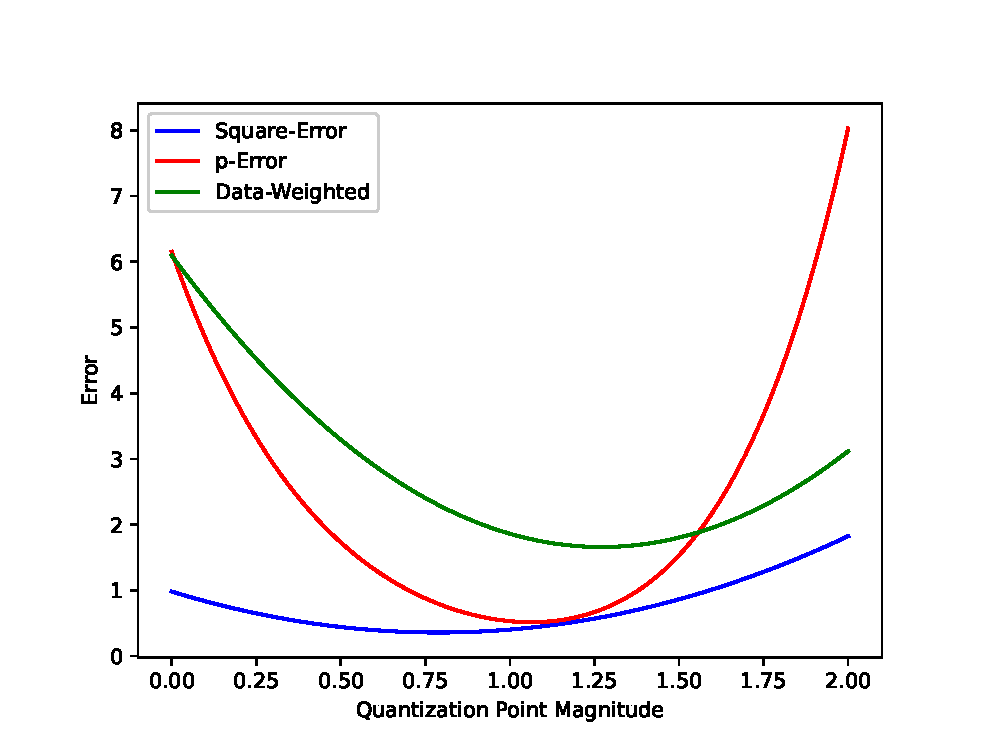
\includegraphics[width=\linewidth]{impact_distortion.eps}%{traces.eps}
	\caption{Impact of distortion functions. $X \sim \mathcal{N}(0,1)$, $p = 5$, $K(x) = \exp(|x|)$.}
	\label{fig:impact_distortion}
\end{figure}

Fig.~\ref{fig:impact_distortion} plots the impact on the true distortion metric for a Gaussian source $X \sim \mathcal{N}(0,1)$ for three scenarios: $D_{\mathrm{SE}}$; $D_p$ in (\ref{eq:p_norm}) with $p = 5$; and the weighted distortion function in (\ref{eq:weight_distort}) with $K(x) = \exp(|x|)$. Observe that the optimal quantization point magnitude, $B$, differs significantly in each of the three scenarios. As such, a quantizer based on $D_{\mathrm{SE}}$ leads to performance reduction with a mismatched distortion function. On the other hand, if the target distortion function is known, it can be utilized to construct a tailored quantizer.

\section{Risk-Averse $1$-Bit Quantization}

Fig.~\ref{fig:impact_distortion} highlights that design of a quantizer based on an approximation mean distortion criterion can lead to a significant performance reduction. In this section, we develop a new design strategy for $1$-bit quantization to account for uncertainty in the distortion function.

\subsection{Proposed Criteria}

Consider a family $\mathcal{D} = \{D_n: n \in \mathcal{N}\}$ of distortion functions $D_n: \mathbb{R}^d \times \mathbb{R}^d \rightarrow \mathbb{R}_+$ index by $n \in \mathcal{N}$. Elements in the index set $\mathcal{N}$ can correspond to different weighting functions $K$ for the weighted distortion function in (\ref{eq:weight_distort}), or values of $p$ in the case of $p$-norm distortion function (\ref{eq:p_norm}). 

Suppose there is a prior distribution $P_N$ on the index set $\mathcal{N}$; i.e., prior information about the target distortion function. In this case, it is natural to construct a quantizer via
\begin{align}\label{eq:quant_prior}
	\min \mathbb{E}_{N,\mathbf{X}}[D_N(\mathbf{X},Q(\mathbf{X}))].
\end{align}
The problem (\ref{eq:quant_prior}) corresponds to Bayesian robust quantizer design \cite{Vempaty2014quantizer}. However, (\ref{eq:quant_prior}) is intractable in general and also requires reliable knowledge of the prior distribution $P_N$. As such, it is necessary to consider tractable approximations. 

The simplest, but widely utilized, approximation is to ignore knowledge of $P_N$ and simply choose a reference distortion function $D_{\mathrm{ref}} \in \mathcal{D}$; e.g., $D_{\mathrm{ref}} = D_{\mathrm{SE}}$. An alternative approach is to observe that 
\begin{align}
	&\mathbb{E}_{N,\mathbf{X}}[D_N(\mathbf{X},Q(\mathbf{X}))]\notag\\
	&= \mathbb{E}_N\left[\int_0^{\infty} \mathbb{P}(D_N(\mathbf{X},Q(\mathbf{X})) > u|N)\mathrm{d}u\right]\notag\\
	&= \int_0^{\infty} \mathbb{E}_N[\mathbb{P}(D_N(\mathbf{X},Q(\mathbf{X})) > u|N)]\mathrm{d}u,
\end{align}
which follows from the fact that the expectation of a real valued random variable $Z$ satisfies $\mathbb{E}[Z] = \int_0^{\infty} \mathbb{P}(Z > u)\mathrm{d}u$. 

Let $h: [0,1] \rightarrow [0,1]$ be a concave function satisfying $h(0) = 0$ and $h(1) = 1$, which implies that $h(w) \geq w,~w \in [0,1]$. It follows that
\begin{align}
	&\mathbb{E}_N[\mathbb{P}(D_N(\mathbf{X},Q(\mathbf{X})) > u|N)]\notag\\
	&\leq \mathbb{E}_N\left[h\left(\mathbb{P}(D_N(\mathbf{X},Q(\mathbf{X})) > u|N)\right)\right]
\end{align}
for all $u \in [0,\infty)$. A conservative estimate of $\mathbb{E}_{N,\mathbf{X}}[D_N(\mathbf{X},Q(\mathbf{X}))]$ is then given by 
\begin{align}
	&\mathbb{E}_{N,\mathbf{X}}[D_N(\mathbf{X},Q(\mathbf{X}))]\notag\\ 
	&\leq \int_0^{\infty} \mathbb{E}_N\left[h\left(\mathbb{P}(D_N(\mathbf{X},Q(\mathbf{X})) > u|N)\right)\right]\mathrm{d}u.
\end{align}
To remove dependence on the prior $P_N$, we make the approximation 
\begin{align}\label{eq:h_approx}
	&\mathbb{E}_N\left[h\left(\mathbb{P}(D_N(\mathbf{X},Q(\mathbf{X})) > u|N)\right)\right]\notag\\
	&\approx h(\mathbb{P}(D_{\mathrm{ref}}(\mathbf{X},Q(\mathbf{X})) > u)).
\end{align}
This approximation corresponds to the standard approach for mean distortion criteria in the case $h(w) = w,~w \in [0,1]$. Nevertheless, unlike the standard approximation, the approximation in (\ref{eq:h_approx}) can be made arbitrarily accurate by setting $h(w) \approx 1$ for all $w \in [0,1]$. 

The quantity 
\begin{align}
	\rho(D_{\mathrm{ref}}(\mathbf{X},Q(\mathbf{X}))) = \int_0^{\infty} h(\mathbb{P}(D_{\mathrm{ref}}(\mathbf{X},Q(\mathbf{X})) > u))\mathrm{d}u
\end{align}
is a form of \textit{risk measure} \cite{Serada2010distortion}. The impact of choosing $h(w) \geq w$ is a higher cost associated to large values of $D_{\mathrm{ref}}(\mathbf{X},Q(\mathbf{X}))$. Quantizers corresponding to the solution of 
\begin{align}\label{eq:risk_criterion}
	\min_{Q,\mathcal{Y}} 	\rho(D_{\mathrm{ref}}(\mathbf{X},Q(\mathbf{X})))
\end{align} 
are therefore \textit{risk averse}. 

We propose to utilize the criterion in (\ref{eq:risk_criterion}) to design $1$-bit quantizers in the presence of uncertainty in the distortion function (or the data distribution $P_{\mathbf{X}}$, as discussed in Sec.~\ref{sec:p_X_uncertainty}). In contrast to standard goal-oriented compression schemes, instead of assuming that the distortion function $D_{\mathrm{ref}}$ is perfectly adapted to a task, we incorporate robustness to uncertainty in the distortion function via $h$. In the sequel, we design optimal $1$-bit quantizers with risk measure criteria by solving (\ref{eq:risk_criterion}). 

\subsection{Optimal $1$-Bit Quantization}

To obtain an optimal $1$-bit quantizer, it is necessary to select both the reproduction set $\mathcal{Y} = \{\mathbf{y}_1,\mathbf{y}_2\} \subset \mathbb{R}^d$, and the quantization function $Q: \mathbb{R}^d \rightarrow \mathcal{Y}$. We first consider the quantization function $Q$. 

Let $\mathcal{Y} = \{\mathbf{y}_1,\mathbf{y}_2\}$ be fixed and $Q: \mathbb{R}^d \rightarrow \mathcal{Y}$ be arbitrary. Observe that 
\begin{align}
	&\int_0^{\infty} h\left(\mathbb{P}(D_{\mathrm{ref}}(\mathbf{X},Q(\mathbf{X})) > u)\right)\mathrm{d}u\notag\\
	&\int_0^{\infty} h\left(\mathbb{P}\left(\min_{\hat{\mathbf{x}} \in \{\mathbf{y}_1,\mathbf{y}_2\}} D_{\mathrm{ref}}(\mathbf{X},\hat{\mathbf{x}}) > u\right)\right)\mathrm{d}u
\end{align}
since for each $u \geq 0$, 
\begin{align}
	\mathbb{P}(D_{\mathrm{ref}}(\mathbf{X},Q(\mathbf{X})) > u) \geq \mathbb{P}\left(\min_{\hat{\mathbf{x}} \in \{\mathbf{y}_1,\mathbf{y}_2\}} D_{\mathrm{ref}}(\mathbf{X},\hat{\mathbf{x}}) > u\right),
\end{align}
and $h$ is a monotonically non-decreasing function. As such, the optimal quantization function is given by 
\begin{align}
	Q^*(\mathbf{x}) = \min_{\hat{\mathbf{x}} \in \{\mathbf{y}_1,\mathbf{y}_2\}} D_{\mathrm{ref}}(\mathbf{X},\hat{\mathbf{x}}).
\end{align} 
Note that the optimal quantization function is the same as for the mean distortion criterion corresponding to $h(w) = w$. 

The optimal reproduction set $\mathcal{Y}$ is therefore given by 
\begin{align}\label{eq:opt_y}
	\min_{\mathbf{y}_1,\mathbf{y}_2 \in \mathbb{R}^d} \int_0^{\infty} h\left(\mathbb{P}\left(\min_{\hat{\mathbf{x}} \in \{\mathbf{y}_1,\mathbf{y}_2\}} D_{\mathrm{ref}}(\mathbf{X},\hat{\mathbf{x}}) > u\right)\right)\mathrm{d}u. 
\end{align}
Unlike for mean distortion criteria, a solution to (\ref{eq:opt_y}) cannot be obtained via a Lloyd-type algorithm \cite{Linde1980algorithm} due to the non-linearity introduced by $h$. To obtain a solution we exploit a global optimization method. In particular, we utilize the cross-entropy method with a Gaussian sampling \cite{Botev2013cross}. Pseudocode for the algorithm\footnote{Code to implement the algorithm along with parameters for the cross-entropy method are available at \url{https://github.com/malcolmalexegan/risk_averse_quantization/tree/master}.} is given in Alg.~\ref{alg:optimization}.

\begin{algorithm}
	\caption{Quantizer Optimization Algorithm}\label{alg:optimization}
	\begin{algorithmic}[1]
		\STATE \textbf{Input:} Maximum number of iterations $T_{\max}$, samples  $\{\mathbf{x}_i\}_{i=1}^S$ from $P_{\mathbf{X}}$, samples for CEM $N$, reference distortion function $D_{\mathrm{ref}}$, risk measure parameter function $h$ in (\ref{eq:risk_criterion}), initial search parameters $\boldsymbol{\mu} \in \mathbb{R}^2$, $\sigma \in \mathbb{R}_+$. \STATE Initialize $t = 0$, $\mathcal{Y}_{\mathrm{best}}$, and $\rho_{\mathrm{best}} = \infty$. 
		\FOR{$t < T_{\max}$}
		\STATE $t \leftarrow t+1$.
		\STATE Sample quantizers $\mathcal{Y}_i \sim \mathcal{N}(\boldsymbol{\mu},\sigma^2\mathbf{I}),~i = 1,\ldots,N$.
		\STATE Estimate risk measure $\rho_i$ in (\ref{eq:risk_criterion}) from data $\{\mathbf{x}_i\}_{i=1}^S$ for each $\mathcal{Y}_i,~i = 1,\ldots,N$.
		\FOR {$i = 1,\ldots,N$}
		\IF{$\rho_i < \rho_{best}$}
		\STATE $\rho_{\mathrm{best}} \leftarrow \rho_i$, $\mathcal{Y}_{\mathrm{best}} \leftarrow Y_i$.
		\ENDIF
		\STATE Update $\boldsymbol{\mu},\sigma$ via \cite[Algorithm 4.1 Eq. (19-21)]{Botev2013cross}.
		\ENDFOR
		\ENDFOR
		\STATE \textbf{Output:} $\mathcal{Y}_{\mathrm{best}}$.
	\end{algorithmic}
\end{algorithm}

\section{Numerical Results}

In rare-event estimation with scalar measurements, such as extreme temperature events, it is desirable to reduce the distortion associated to samples with large values. This can be modeled via a distortion function $K(X)|X - \hat{X}|^2$ with $K$ monotonically increasing. In this case, misspecification of $K$, such as the choice $D_{\mathrm{ref}}(X,\hat{X}) = |X - \hat{X}|^2$, can lead to poor performance.

We investigate our $1$-bit quantization strategy using temperature data from the Twin House Experiment \cite{Kersken2020}. In this setting, $1$-bit quantization reduces the communication requirements of low-power sensors, relevant for classification of extreme temperature events condition monitoring applications. We investigate the design of quantizers based on the criteria 
\begin{align}\label{eq:risk_power}
	\rho_{\alpha} = \int_0^{\infty} \left(\mathbb{P}(D_{\mathrm{SE}}(X,\hat{X}) > u)\right)^{\alpha}\mathrm{d}u,~\alpha \in (0,1].
\end{align} 
When $\alpha = 1$, $\rho = \mathbb{E}[D_{\mathrm{SE}}(X,\hat{X})]$, while for small values of $\alpha$, the quantizer attempts to reduce the distortion for lower probability events. This has the byproduct of reducing quantization errors for extreme temperature events. Fig.~\ref{fig:time_series} shows the temperature time series and corresponding quantized data obtained from the optimized quantizer with $\alpha = 0.1$.

Table~\ref{table:Twin_house} shows the optimized quantizer using Alg.~\ref{alg:optimization}, threshold, and corresponding values of risk measures with varying $\alpha$. Here, $\rho_{\alpha}$ denotes the value of the risk measure in (\ref{eq:risk_power}) with parameter $\alpha$. Observe that quantization levels $y_1,y_2$ in $\mathcal{Y}$ for optimized quantizer increase as $\alpha$ decreases. In other words, increasing the cost associated with low probability events associated with extreme events leads to quantization levels that approach the values of the extreme events.  

\begin{figure}
	\centering
	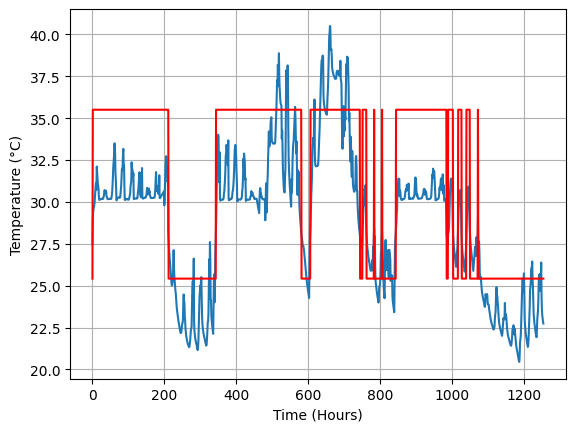
\includegraphics[width=\linewidth]{time_series_FIN.png}%{traces.eps}
	\caption{Temperature time series from the Twin House Experiment \cite{Kersken2020} (sensor in the living room at a height of 10cm) and corresponding quantization based on $\rho_{0.1}$, corresponding to $\alpha = 0.1$ in (\ref{eq:risk_power}).}
	\label{fig:time_series}
\end{figure}

\begin{table}[h]
	\centering
	\caption{Risk-Aware Quantization}
	\begin{tabular}{|c|c|c|c|c|c|c|}
		\hline
		$\alpha$ & $y_1$ & $y_2$ & Threshold &  $\rho_1$ & $\rho_{0.5}$ &  $\rho_{0.1}$ \\
		\hline
		$1$ & $24.44$ & $31.74$ & $28.09$ & $\mathbf{5.44}$ & $15.17$ & $52.57$ \\
		\hline
		$0.5$ & $24.77$ & $33.43$ & $29.1$ & $7.04$ & $\mathbf{12.60}$ & $34.72$ \\
		\hline
		$0.1$ & $25.42$ & $35.51$ & $30.46$ & $12.14$ & $16.88$ & $\mathbf{23.15}$ \\
		\hline
	\end{tabular}
\label{table:Twin_house}
\end{table}

\section{Conclusion}

Goal-oriented compression relies on knowledge of an application-dependent distortion function. In practice, there may be uncertainty in the choice of this distortion function. In this paper, we have proposed a new approach to robust quantization to cope with both uncertainty in the data distribution and the distortion function. We establish a connection between robust quantization and risk measures, which leads to new criteria. To optimize the quantizer based on risk measure criteria, we apply the cross-entropy method. Our approach is illustrated for environmental monitoring data from the Twin House Experiment \cite{Kersken2020}.


\bibliographystyle{IEEEtran}
\bibliography{1_bit_quantization.bib}


\end{document}